\documentclass[xcolor=table, 11pt, aspectratio=169]{beamer}

% \usepackage{arev}
\usepackage{amsmath,amssymb,amscd,physics}
\usepackage{dsfont}
\usepackage{mathrsfs}
\usepackage{yfonts}
\usepackage{bm}
\usepackage{graphicx}
\usepackage{tabularx}
\usepackage{animate}
\usepackage{listings}
\usepackage{pifont}
\usepackage{booktabs}
\usepackage{multirow}
\usefonttheme[onlymath]{serif}

%\usepackage{mathtools}
%\usepackage{ifthen}

\usepackage{xeCJK}
%\usepackage{fontspec}
\newfontfamily\cjkfont{FZHei-B01}
%\setCJKmainfont{PingFang SC}
\newcolumntype{x}{>{\centering\arraybackslash}X}
\renewcommand{\arraystretch}{1.5}
\newcommand{\uone}{\mathrm U(1)}
\DeclareMathOperator{\img}{img}
\lstset{language=GAP}

\usepackage{tikz}
	\usetikzlibrary{calc}
	\usetikzlibrary{arrows,shapes, positioning, matrix}
	\usetikzlibrary{decorations.markings}
	\tikzset{>=stealth}
	\tikzstyle arrowstyle=[scale=1]
	\tikzstyle directed=[postaction={decorate,decoration={markings,
 	   mark=at position .15 with {\arrow[arrowstyle]{stealth}}}}]
\tikzstyle string=[thick,postaction={decorate,decoration={markings,
    mark=at position .55 with {\arrow[arrowstyle]{stealth}}}}]
\tikzstyle dual_string=[dashed,postaction={decorate,decoration={markings,
    mark=at position .55 with {\arrow[arrowstyle]{stealth}}}}]

\tikzstyle dw=[thick,postaction={decorate,decoration={markings,
    mark=at position 1 with {\arrow[arrowstyle]{stealth}}}}]
\tikzstyle group=[mbg]
\newcommand*{\halfway}{0.5*\pgfdecoratedpathlength+.5*8pt}\tikzstyle arrowstyle=[scale=1]
\newcommand*{\halfwayb}{0.5*\pgfdecoratedpathlength}
\tikzstyle arrowstyle=[scale=1]
\tikzstyle fermion=[thick,postaction={decorate},decoration={markings,
    mark=at position \halfway with {\arrow[arrowstyle]{latex}}}]
\tikzstyle fermion2=[thick,postaction={decorate},decoration={markings,
        mark=at position \halfwayb with {\arrow[arrowstyle]{latex}}}]

\usepackage{pgffor}
\newcommand{\mb}[1]{\mathbf{#1}}
\renewcommand{\cal}[1]{\mathcal{#1}}

\newcommand{\ag}[2]{#1_\mb{#2}}
\newcommand{\cohosub}[1]{\scalebox{0.72}{\textswab{#1}}}
\newcommand{\cohosubsub}[1]{\scalebox{0.6}{\textswab{#1}}}
\newcommand{\coho}[1]{\textswab{#1}}

%\DeclareMathOperator{\tr}{Tr}
\DeclareMathOperator{\im}{Im}
\DeclareMathOperator{\re}{Re}

\mode<presentation>
{
  %\usetheme{Warsaw}
  % or ...
  %\useoutertheme{rectangle}
  \setbeamertemplate{frametitle}[default][center]
  \defbeamertemplate{itemize item}{flat}{\begin{pgfpicture}{-1ex}{0ex}{1ex}{2ex}
      \pgfpathcircle{\pgfpoint{0pt}{.6ex}}{0.6ex}
      \pgfusepath{fill}
    \end{pgfpicture}%
  }
  \defbeamertemplate{itemize subitem}{flat}{\footnotesize\raise0.5pt\hbox{\textbullet}}
  \defbeamertemplate{itemize subsubitem}{flat}{\footnotesize\raise0.5pt\hbox{\textbullet}}

  %\useinnertheme{circles}
  \setbeamertemplate{items}[flat]
  \setbeamertemplate{sections/subsections in toc}[circle]
  \setbeamertemplate{blocks}[rounded]
  \setbeamertemplate{title page}[default][colsep=-4bp,rounded=true]
  \setbeamertemplate{part page}[default][colsep=-4bp,rounded=true]
  \setbeamercovered{transparent}
  %\usecolortheme{spruce}
  %\definecolor{THU}{RGB}{116,61,130}
  \definecolor{mbg}{RGB}{0,0,160}
  \setbeamercolor*{palette primary}{fg=white,bg=mbg}
  \setbeamercolor*{titlelike}{parent=palette primary}
  \setbeamercolor*{structure}{fg=mbg}
  \setbeamercolor{frametitle}{fg=white,bg=mbg}
  % or whatever (possibly just delete it)
  \setbeamercolor{block title}{bg=mbg,fg=white}
  \setbeamercolor{block body}{bg=mbg!15}


  \addtobeamertemplate{navigation symbols}{}{ \hspace{1em}%
    \usebeamerfont{footline}%
    \insertframenumber / \inserttotalframenumber }
}


%\usepackage[english]{babel}
% or whatever

%\usepackage[latin1]{inputenc}
% or whatever

%\usepackage{times}
%\usepackage[T1]{fontenc}
% Or whatever. Note that the encoding and the font should match. If T1
% does not look nice, try deleting the line with the fontenc.

\title[DMRG and Fuzzy Sphere] % (optional, use only with long paper titles)
{Multi-target density matrix renormalization group for 3D CFTs on the fuzzy sphere}

\author[Y Qi] % (optional, use only with lots of authors)
{Yang~Qi}
% - Give the names in the same order as the appear in the paper.
% - Use the \inst{?} command only if the authors have different
%   affiliation.

\institute[Fudan] % (optional, but mostly needed)
{Department of Physics, Fudan University}
% - Use the \inst command only if there are several affiliations.
% - Keep it simple, no one is interested in your street address.

%\date{2016 Annual Meeting of Fudan CFTPP} % (optional, should be abbreviation of conference name)
%\date{Miniworkshop on Quantum Many-Body Physics, July 29, 2024.}
\date{全国理论物理前沿与交叉科学研讨会, 2026年4月18日.}
% - Either use conference name or its abbreviation.
% - Not really informative to the audience, more for people (including
%   yourself) who are reading the slides online

\subject{Theoretical Physics}
% This is only inserted into the PDF information catalog. Can be left
% out.



% If you have a file called "university-logo-filename.xxx", where xxx
% is a graphic format that can be processed by latex or pdflatex,
% resp., then you can add a logo as follows:

\pgfdeclareimage[height=1cm]{university-logo}{../resources/fudan}
\logo{\pgfuseimage{university-logo}}

\AtBeginSection[]
{
\begin{frame}{Outline}
%	\begin{columns}
%		\begin{column}[t]{.45\textwidth}
%		\begin{center}
%			
\includegraphics[height=4cm]{toys}
%		\end{center}
%	\end{column}
%	\begin{minipage}[t][0.5\textheight]{0.55\textwidth}
      \tableofcontents[currentsection]
%    \end{minipage}\hfill
%	\end{columns}
\end{frame}
}


% Delete this, if you do not want the table of contents to pop up at
% the beginning of each subsection:

\begin{document}

\begin{frame}
  \titlepage
\end{frame}

\begin{frame}{Collaborators}
  \begin{itemize}
  \item Jin-Xiang Hao (郝进翔): Fudan University.
  \item Zheng Zhu (朱征): Kavli Institute of Theoretical Sciences, UCAS.
\end{itemize}
%\vspace{4em}
\begin{center}
  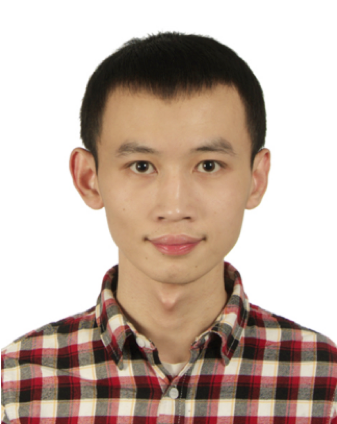
\includegraphics[height=3.5cm]{../people/zhengzhu}~~~~
  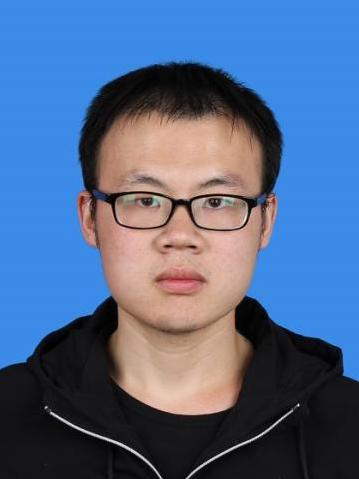
\includegraphics[height=3.5cm]{../people/jxhao}
\end{center}
\begin{enumerate}
\item J-X Hao, Z Zhu and YQ, arXiv:2601.18648;
\item J-X Hao and YQ, to appear.
\end{enumerate}
\end{frame}

\begin{frame}{Outline}
%	\begin{columns}
%		\begin{column}[t]{.45\textwidth}
%		\begin{center}
%			
\includegraphics[height=4cm]{toys}
%		\end{center}
%	\end{column}
%	\begin{minipage}[t][0.5\textheight]{0.55\textwidth}
      \tableofcontents
%    \end{minipage}\hfill
%	\end{columns}
\end{frame}

% Section 1: Introduction
\section{Introduction to 3D CFTs and Fuzzy}
% Slide 3: The Challenge of 3D CFTs
\begin{frame}{The Challenge of 3D CFTs}
    \begin{itemize}
        \item \textbf{Conformal Field Theories (CFTs)} are fundamental to understanding continuous quantum phase transitions and quantum gravity.
        \item While 2D CFTs are heavily constrained by the infinite-dimensional Virasoro algebra, 3D CFTs possess finite-dimensional global conformal symmetry.
        \item \textbf{The Core Problem:} Extracting precise conformal data (e.g., scaling dimensions of primary operators) in 3D strongly interacting systems is highly challenging.
        \item Traditional lattice models suffer from finite-size effects and loss of conformal symmetry at the lattice scale.
    \end{itemize}
\end{frame}

\begin{frame}{Fuzzy Sphere Regularization}
  \begin{itemize}
  \item \textbf{Concept:} Construct a lattice model by projecting spatial degrees of freedom onto the Lowest Landau Level (LLL) of a spherical geometry with a magnetic monopole.
  \item Effective system size: $N\propto \text{monopole strength}$.
        %\item \textbf{Hamiltonian Structure:}
        %\begin{equation*}
        %    H = \frac{1}{2m_e R^2} (L^2 - s^2)
        %\end{equation*}
        %where $s$ is the monopole strength and $L$ is the angular momentum.
  \item \textbf{Advantage:} This setup preserves the $SO(3)$ rotational symmetry of the sphere precisely. It is believed that this allows the system to flow to conformal fixed-point quickly.
  \item Accurate conformal weights from small system sizes: $N=16$ gives $\Delta(\epsilon)=1.414$ vs $1.413$ from bootstrap.
  \item Wei Zhu, et al, PRX 2023.
  \end{itemize}
\end{frame}

\begin{frame}{State-Operator Correspondence}
  \begin{center}
    \includegraphics[width=\textwidth]{state-op}
  \end{center}
  \begin{itemize}
  \item Each eigenstate $|\mathcal O\rangle$ corresponds to an operator $\mathcal O$ in the CFT.
  %\item Ground state $|0\rangle$ maps to the identity $1$.
  \item Symmetry quantum number (angular momentum, global symmetry, etc) of $|\psi\rangle$ is the same as the operator $\psi$.
  \item Energy of $|\psi\rangle$ is proportional to the conformal weight of $\psi$, with an unknown factor.
  \end{itemize}
\end{frame}

% Slide 4: The Exponential Wall
\begin{frame}{The Bottleneck: Exact Diagonalization (ED)}
  \begin{center}
    \includegraphics[width=.7\textwidth]{cf-tower}
  \end{center}
  \begin{itemize}
  \item ED is suitable for the task because it can access excited states corresponding to different primary/decendent fields.
  \item \textbf{The Limitation:} ED is restricted by the \textit{exponential wall} of the Hilbert space.
  \item Finite-size effect hinders the identification of higher-energy primary operators.
  %\item Can we do better?
  \end{itemize}
\end{frame}

% Section 2: Methodology
\section{Methodology: Fuzzy Sphere \& DMRG}
% Slide 5: Fuzzy Sphere Regularization

% Slide 7: Density Matrix Renormalization Group (DMRG)
\begin{frame}{Overcoming the Limit: DMRG}
  \begin{block}{Why DMRG?}
    The Density Matrix Renormalization Group (DMRG) bases on Matrix Product States (MPS).
    \begin{itemize}
    \item Has been successful in studying ground states of interacting models on fuzzy-sphere geometry.
    \item Does not face sign problems.
    \item Expected to work on moderate-size systems beyond the reach of ED.
    \end{itemize}
  \end{block}
  Challenge: how to access excited states?
  \begin{itemize}
  \item \textbf{Using Symmetries:} We can independently target the lowest energy states in specific symmetry sectors.
  \item \textbf{Multi-target DMRG:} Use boundled MPS and block Lanczos procedure.
  \end{itemize}
\end{frame}
  
\begin{frame}{Targeting Symmetry Sectors}
  \begin{columns}
    \column{.4\textwidth}
    \begin{itemize}
    \item Abelian symmetries: $\mathrm{SO}(2)$ and $\mathbb Z_2$. This can be encoded into the MPS.
    \item $\mathrm{SO}(3)$ symmetry: we target the sector of certain $L$ by adding $\bm L^2$ to the Hamiltonian
      \[H = H_0 + \lambda \bm{L}^2.\]
    \end{itemize}
    \column{.6\textwidth}
    \begin{tabular}{|c|c|c|c|c|c|}
      \hline
      \multirow{2}{*}{$\mathbb Z_2$} & \multirow{2}{*}{$l$} & \multicolumn{4}{|c|}{\textbf{operators}} \\
      \cline{3-6}
                                     & & 0 & 1 & 2 & 3\\
      \hline
      \multirow{3}{*}{1} & 0 & $I$ & \alert{$\epsilon$} & $\Box\epsilon$ & \alert{$\epsilon^\prime$} \\
      \cline{2-6}               
                                     & 1 & $\partial_\mu\epsilon$ & $\partial_\mu\Box\epsilon$ & $\partial_\mu\epsilon^\prime$ & $\partial_\mu\Box^2\epsilon$ \\    
      \cline{2-6} 
                                     & 2 & \alert{$T_{\mu\nu}$} & $\partial_\mu\partial_\nu\epsilon$ & $\epsilon_{\nu\rho\mu}\partial_\rho T_{\mu\nu}$ & $\Box T_{\mu\nu}$ \\                                                            
      \hline
      \multirow{3}{*}{-1} & 0 & \alert{$\sigma$} & $\Box\sigma$ & $\Box^2\sigma$ & \alert{$\sigma^\prime$} \\ 
      \cline{2-6}
                                     & 1 & $\partial_\mu\sigma$ & $\partial_\mu\Box\sigma$ & $\partial_{\mu}\sigma_{\mu\nu}$ & $\partial_\mu\Box^2\sigma$ \\  
      \cline{2-6}
                                     & 2 & $\partial_{\mu}\partial_{\nu}\sigma$ & \alert{$\sigma_{\mu\nu}$} & $\Box\partial_\mu\partial_\nu\sigma$ & $\epsilon_{\nu\rho\mu}\partial_\rho\sigma_{\mu\nu}$ \\ 
            \hline
        \end{tabular}
  \end{columns}
\end{frame}
% Slide 8: Advanced DMRG Techniques
\begin{frame}{Advanced DMRG Techniques}
  \begin{block}{Challenges}
    \begin{itemize}
    \item To extract accurate CFT spectra, we must calculate \textit{excited states}.
    \item Standard DMRG penalty methods are inefficient for multiple excitations.
    \end{itemize}
  \end{block}
     
    
    \vspace{0.3cm}
    \textbf{Multi-target DMRG with Block Lanczos (For Ising CFT)}
    \begin{itemize}
    \item Generalizes MPS to a \textit{bundled MPS} with an extra index for excitations.
    \item Block Lanczos procedure updates the orthogonality center, accurately computing multiple low-lying states simultaneously.
    \end{itemize}
    \begin{center}
      \includegraphics[width=.6\textwidth]{mt-mps}
    \end{center}
    
   % \textbf{2. Truncated DMRG Scheme (For GNY CFT)}
    %\begin{itemize}
     %   \item Long-range interactions in fermionic models demand massive memory (Bond dimension $D \sim 20000$).
     %   \item We truncate the bond dimension at high-energy Landau levels (where particle occupation is minimal) to drastically reduce computational cost while maintaining precision.
    %\end{itemize}
\end{frame}

% Section 3: Application I - 3D Ising CFT
\section{Application I: 3D Ising CFT}
% Slide 9: 3D Ising Model on the Fuzzy Sphere
% \begin{frame}{Application I: 3D Ising CFT}
%     \begin{itemize}
%         \item \textbf{Model:} 3D Ising-type interaction projected onto the LLL.
%         \item \textbf{Hamiltonian:}
%         \begin{equation*}
%             H = H_0 + \lambda \vec{L}^2
%         \end{equation*}
%         \item The $\lambda \vec{L}^2$ term is added to penalize states with total angular momentum $l > m_z$, allowing us to isolate states with specific $l = m_z$.
%         \item \textbf{Simulation Details:} Multi-target DMRG up to size $s=15.5$ ($N=32$ orbitals), extracting the lowest 4 states in each $(z=\pm 1, m_z)$ symmetry sector.
%     \end{itemize}
% \end{frame}

\begin{frame}{Results: Conformal Tower of 3D Ising CFT from DMRG}
  \begin{columns}
    \column{.45\textwidth}
    \begin{itemize}
    \item Multi-target DMRG up to size $s=15.5$ ($N=32$ orbitals), extracting the lowest 4 states in each $(z=\pm 1, m_z)$ symmetry sector.
    \item Less tower states than ED, but enough to determine the conformal weights.
    \item Relying on smaller-size ED to confirm CFT.
    \end{itemize}
    \column{.55\textwidth}
    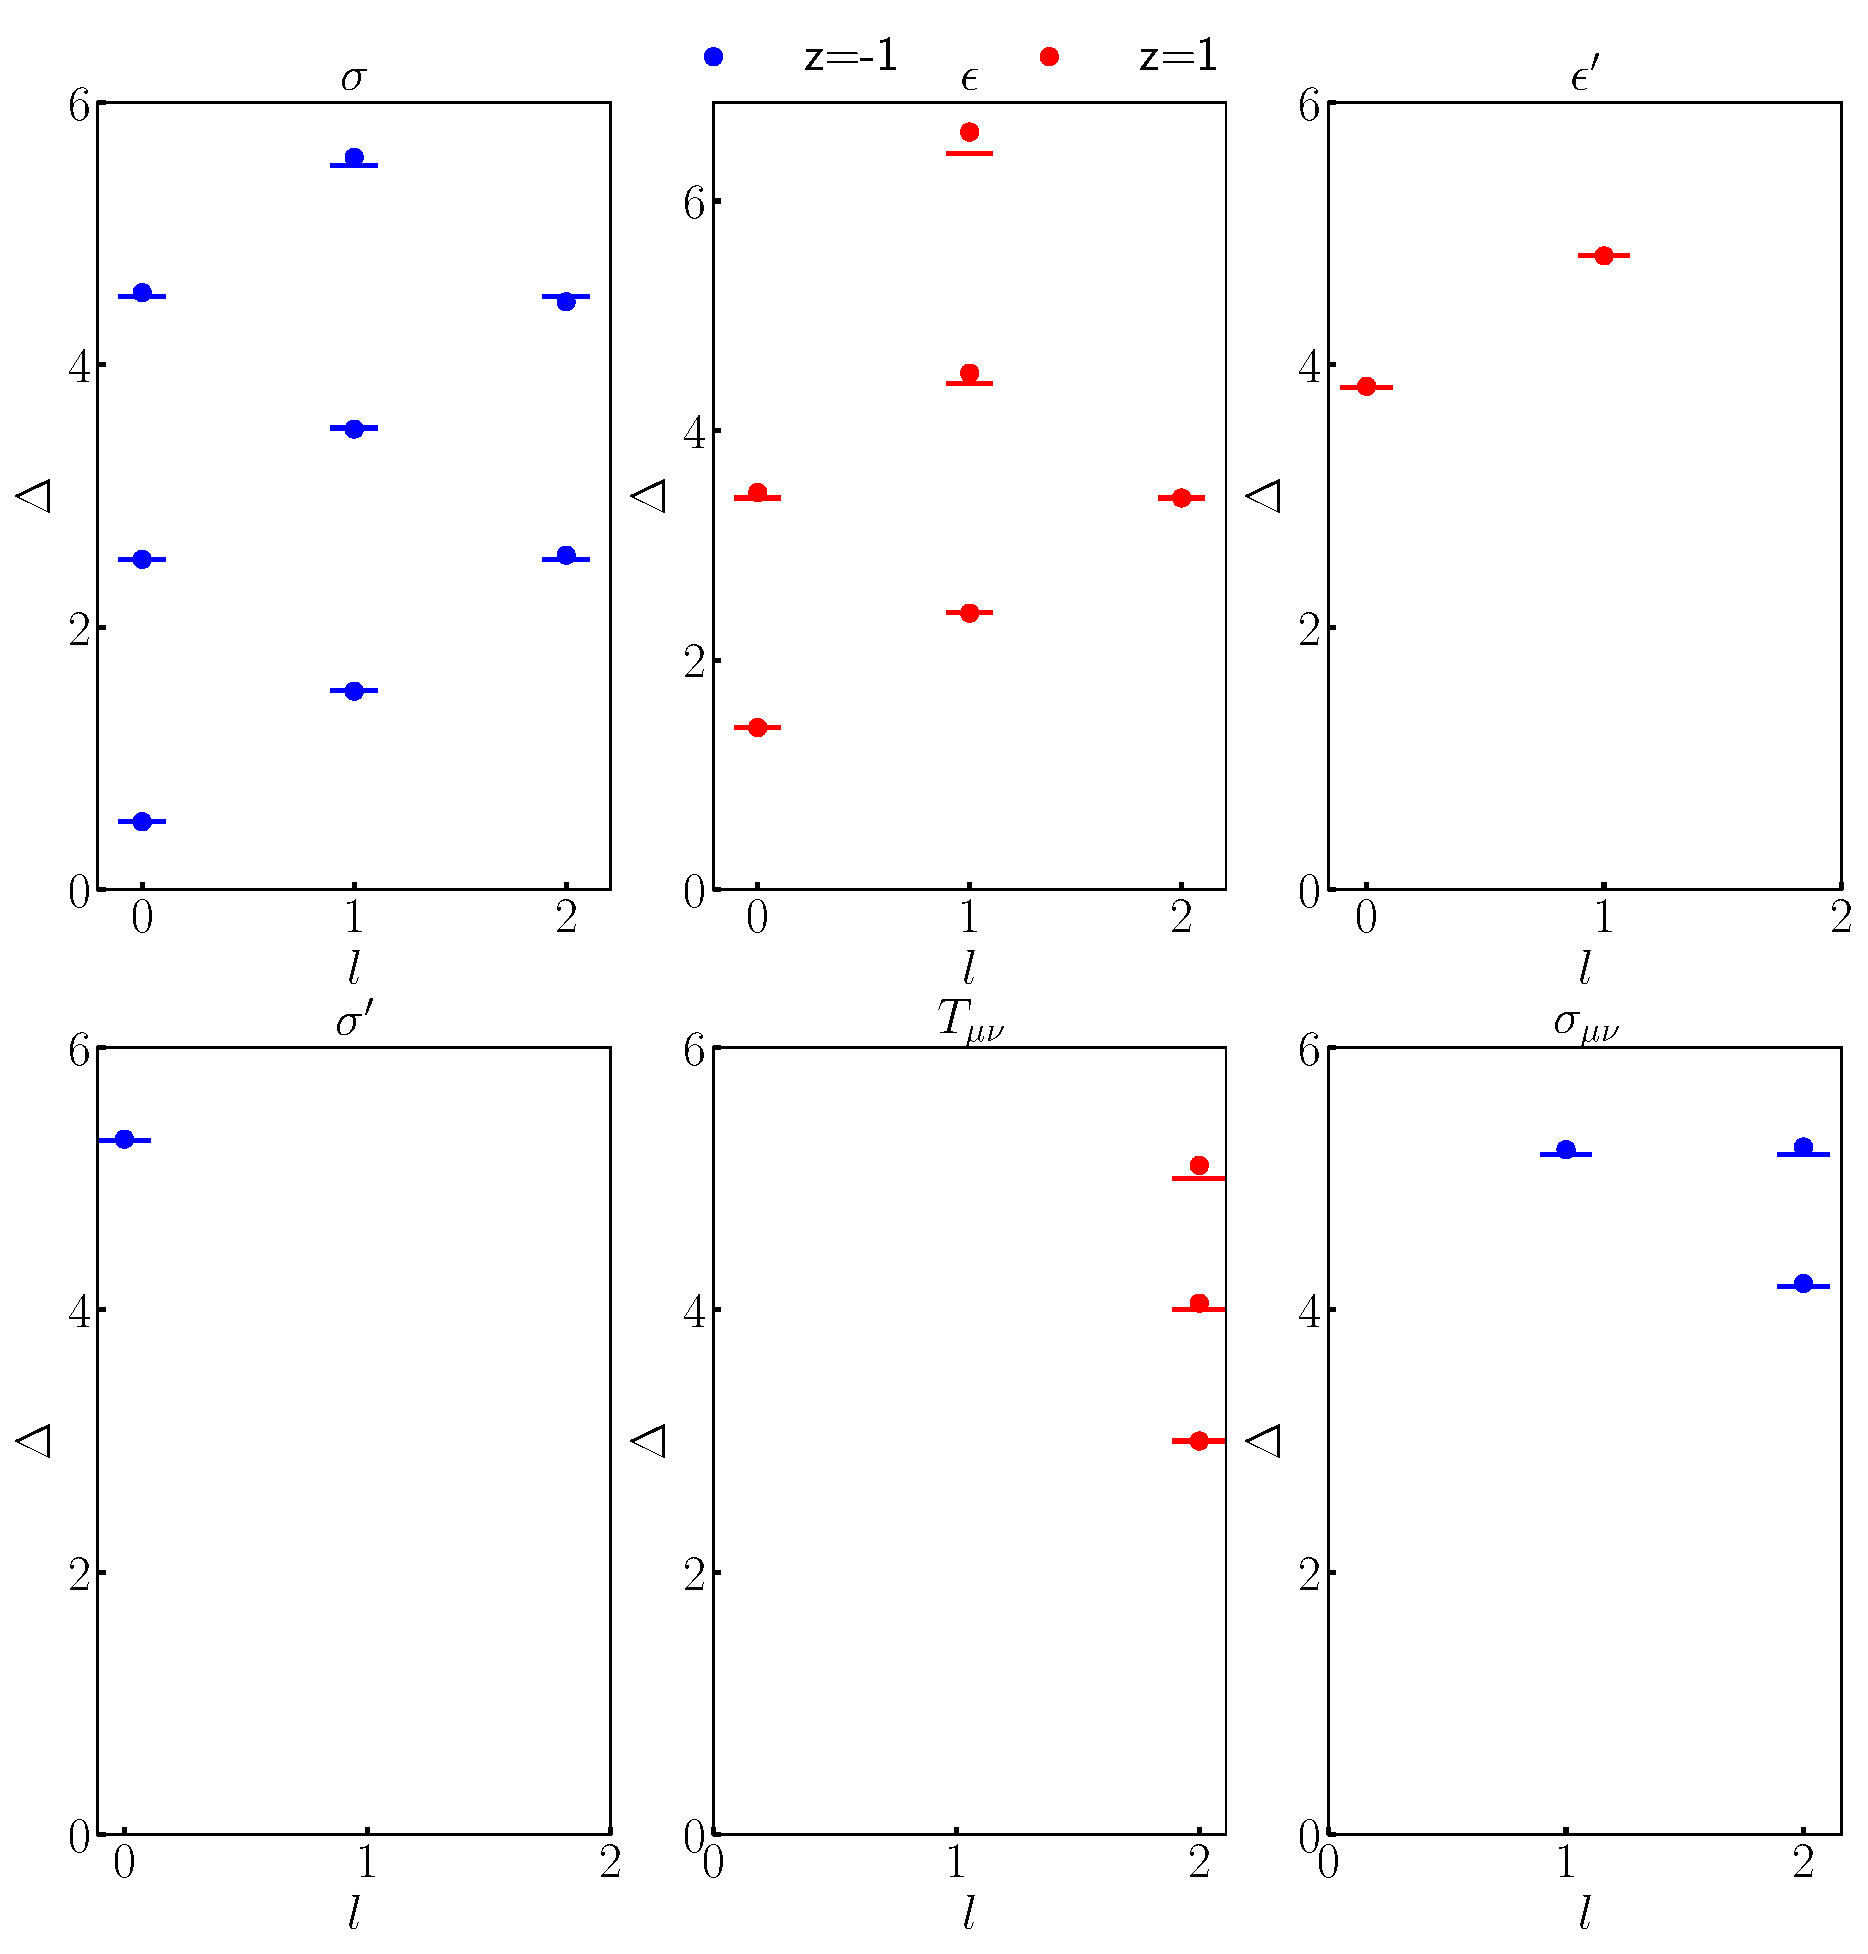
\includegraphics[width=.9\textwidth]{ising-tower}
  \end{columns}
\end{frame}
% Slide 10: Results - 3D Ising CFT
\begin{frame}{Results: 3D Ising CFT Scaling Dimensions}
    \begin{table}[]
        \centering
        \resizebox{\textwidth}{!}{
        \begin{tabular}{lcccccc}
        \toprule
        \textbf{Primary Operators} & $\sigma$ & $\epsilon$ & $\epsilon'$ & $\sigma'$ & $T_{\mu\nu}$ & $\sigma_{\mu\nu}$ \\
        \midrule
        Symmetry $(z, l)$ & $(-1, 0)$ & $(1, 0)$ & $(1, 0)$ & $(-1, 0)$ & $(1, 2)$ & $(-1, 2)$ \\
        \midrule
        \textbf{Bootstrap Benchmark} & 0.518 & 1.413 & 3.830 & 5.291 & 3.00 & 4.180 \\
        \textbf{Fuzzy Sphere (ED, $N=16$)} & 0.524 & 1.414 & 3.838 & 5.303 & 3.00 & 4.214 \\
        \textbf{Fuzzy Sphere (DMRG, $N=32$)} & \textbf{0.519} & \textbf{1.413} & \textbf{3.836} & \textbf{5.299} & \textbf{3.00} & \textbf{4.205} \\
        \bottomrule
        \end{tabular}}
    \end{table}
    \vspace{0.2cm}
    \begin{itemize}
    %\item Multi-target DMRG up to size $s=15.5$ ($N=32$ orbitals), extracting the lowest 4 states in each $(z=\pm 1, m_z)$ symmetry sector.
    %\item Fixing $\Delta(T_{\mu\nu})=3$, and locate the phase transition
    \item Scaling dimensions are linearly proportional to the rescaled energy gaps (normalized by setting energy of $T_{\mu\nu}$ to 3).
    \item \textbf{Conclusion:} DMRG results show significantly reduced errors compared to ED, demonstrating excellent agreement with the conformal bootstrap.
    \end{itemize}
\end{frame}

% Section 4: Application II - 3D GNY CFT
\section{Application II: 3D GNY CFT}

% Slide 6: Dirac Landau Levels (Fermionic Models)
\begin{frame}{Extension to Dirac Landau Levels}
  \begin{columns}
  \column{.6\textwidth}
  \begin{itemize}
  \item To study the \textbf{Gross-Neveu-Yukawa (GNY)} theory, we extend the regularization to Dirac fermions.
  \item Dirac fermion + Hubbard-$U$: from Dirac semimetal to $\mathbb Z_2$ breaking phase (AHE). $\mathbb Z_2$-GNY universality class.\\
    \emph{T. Neupert et al, PRL 2015.}
  %\item Surface states of a 3D topological insulator are described by a 2D Dirac equation on a sphere.
  \item Electrons move on a sphere with a monopole $2\pi$ for spin-up and $-2\pi$ for spin-down. 
  \item The degeneracy of the $(n+1)$-th Landau level is $2(n+1)$.
  \item Difficult to scale up: need to include a full Landau level.
  \end{itemize}
  \column{.4\textwidth}
  \begin{center}
    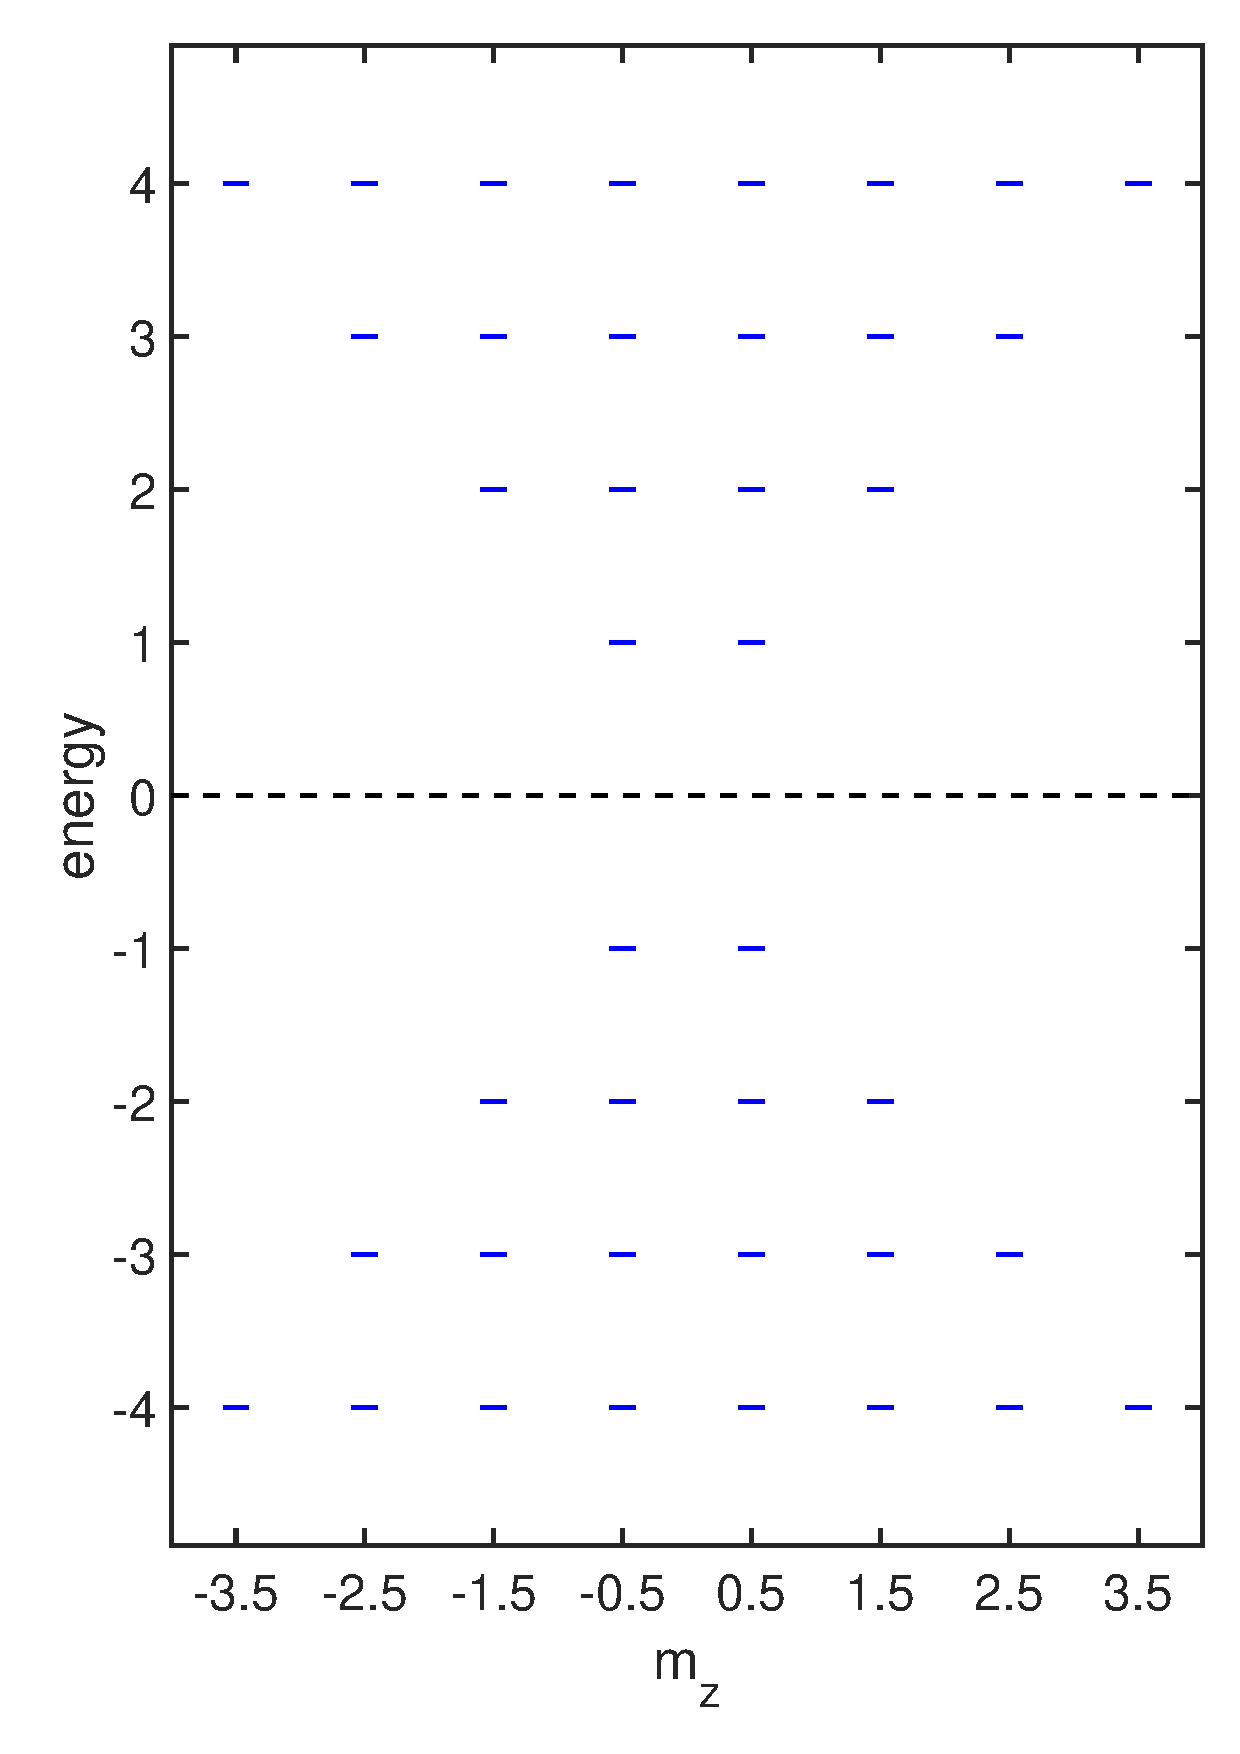
\includegraphics[width=\textwidth]{dirac-energy}
  \end{center}
  \end{columns}
\end{frame}

% % Slide 11: 3D Gross-Neveu-Yukawa Model
% \begin{frame}{Application II: 3D Gross-Neveu-Yukawa (GNY) CFT}
%     \begin{itemize}
%         \item GNY theory describes the topological phase transition in a Chern insulator with 2 fermion flavors.
%         \item \textbf{Interaction:}
%         \begin{equation*}
%             H = H_0 + \int d\Omega_1 d\Omega_2 U(\Omega_1, \Omega_2) \rho_{\uparrow}(\Omega_1)\rho_{\downarrow}(\Omega_2)
%         \end{equation*}
%         \item System undergoes a transition from a gapless phase to a ferromagnetic ordered phase as interaction strength $U$ increases.
%         \item Truncated DMRG is applied, projecting onto the $n_{max} = 3$ Dirac Landau levels to isolate the critical point.
%     \end{itemize}
% \end{frame}

% Slide 12: Results - GNY Phase Transition
% \begin{frame}{Results: Criticality in GNY CFT}
%     \begin{itemize}
%         \item Critical points cannot easily be located using standard Binder cumulant crossings due to size limitations.
%         \item \textbf{Physical Insight:} We use the exact \textit{conformal tower structure} at criticality!
%         \item The critical point $(U_{0c}, U_{1c})$ is determined by tuning parameters until the descendant operator energy $e_2$ strictly obeys $e_1 + 1 = e_2$ (where $e_1$ is the primary operator $\sigma$).
%     \end{itemize}
% \end{frame}

% Slide 13: Results - New Operator Discovery
% \begin{frame}{Results: Multiplets and a New Operator}
%     \begin{block}{Discovery of $J'_\mu$}
%         Analysis of the GNY conformal multiplet structure revealed a previously unreported primary operator $J'_\mu$.
%     \end{block}
%     \vspace{0.2cm}
%     \begin{itemize}
%         \item Unlike the conserved current $J_\mu$, $J'_\mu$ is a \textit{non-conserved} vector operator ($\partial^\mu J'_\mu \neq 0$).
%         \item Scaling dimension analysis ($N=3$ truncation):
%             \begin{itemize}
%                 \item $\sigma$: DMRG $0.64$ (Bootstrap $0.66$)
%                 \item $T_{\mu\nu}$: Fixed at $3.00$
%                 \item $J'_\mu$: Measured at $\sim 2.49$ (Not previously predicted by bootstrap).
%             \end{itemize}
%         \item This highlights the power of numerical Hamiltonian methods to uncover \textit{new structural features} of CFTs missed by analytical methods.
%     \end{itemize} % <--- 修正点：补上了这个闭合标签
%   \end{frame}

\begin{frame}{Inhomogeneous MPS}
  The higher Landau levels are less occupied: not so entangled?
  \begin{center}
    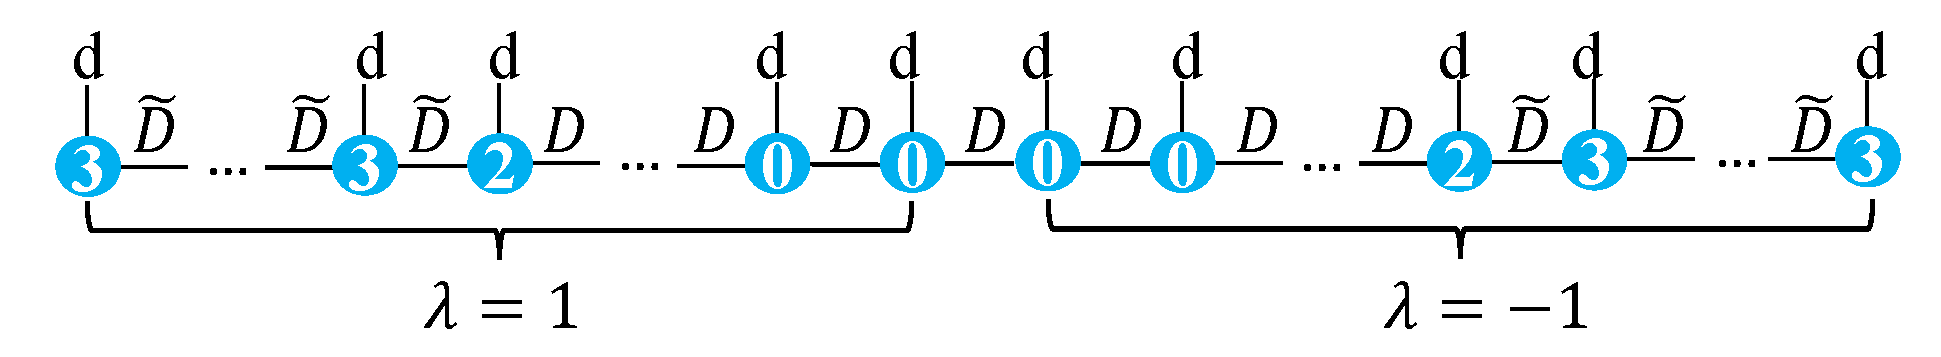
\includegraphics[width=.7\textwidth]{truncateMPS}
    \vspace{2cm}
    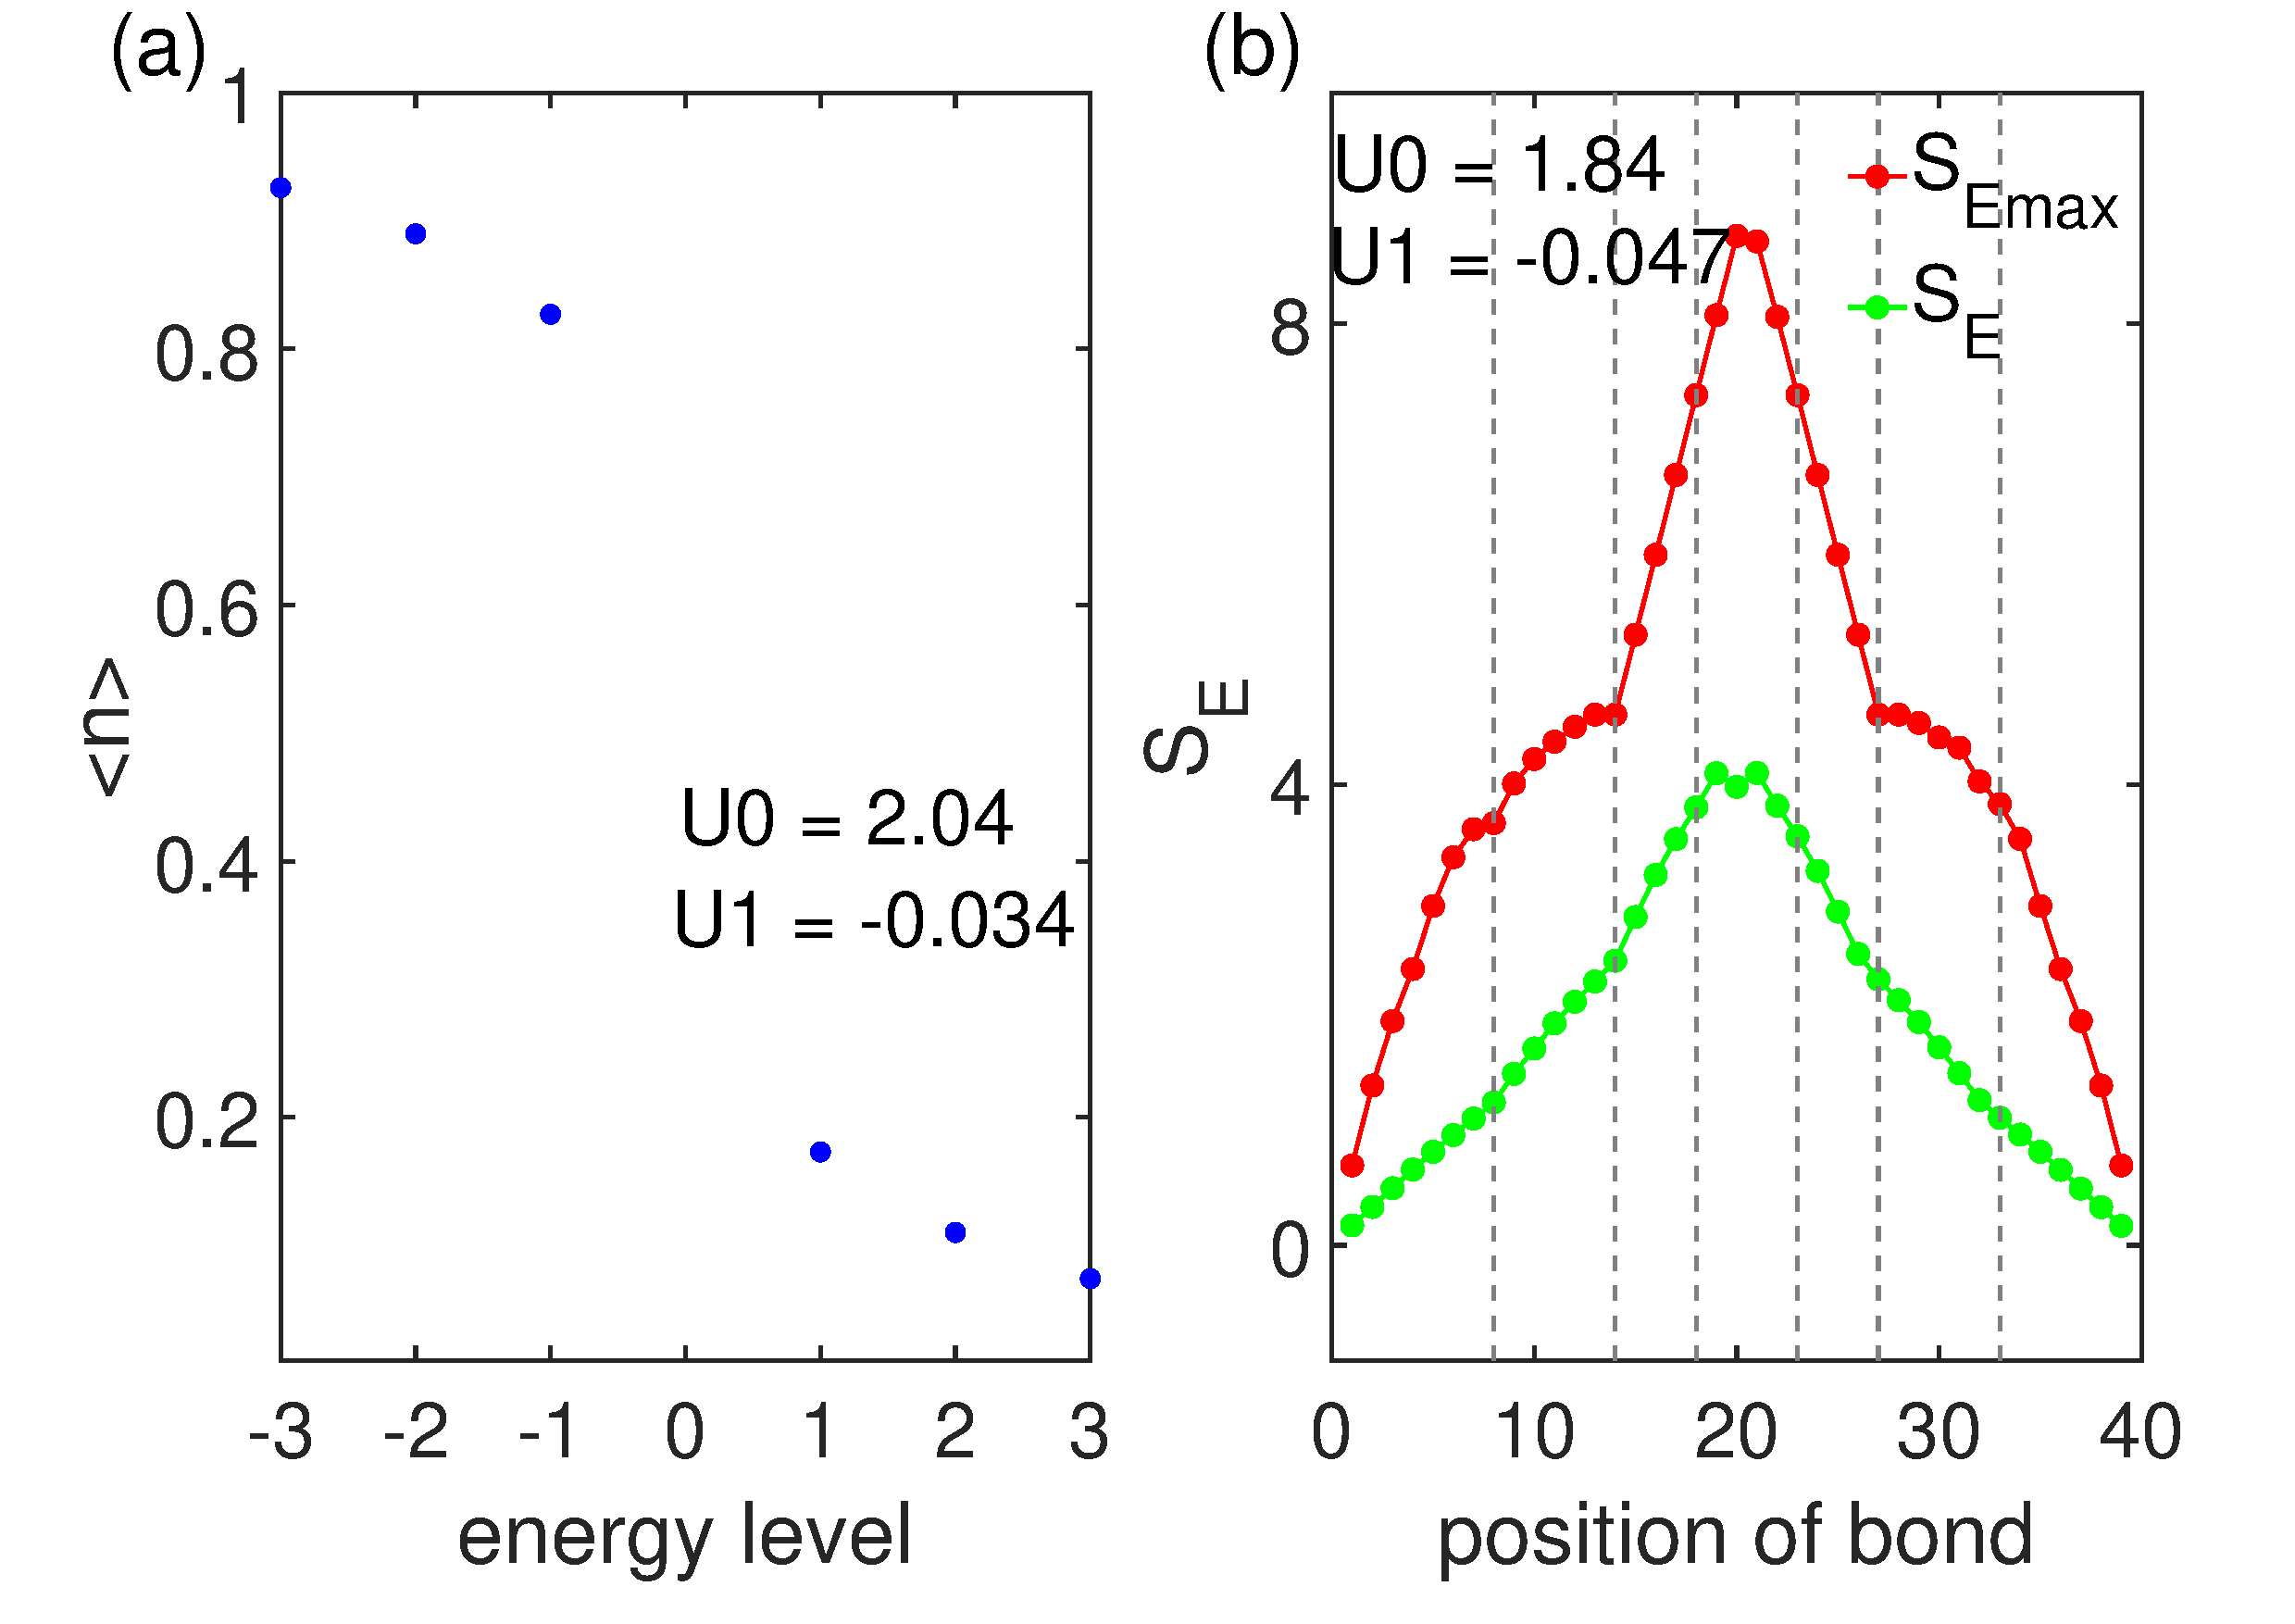
\includegraphics[width=.6\textwidth]{occupy}
  \end{center}
\end{frame}

\begin{frame}{DMRG Results}
      \begin{tabular}{c|c|c|c|c|c|c}
      \hline
      \textbf{$\hat{O}_{primary}$} & $\sigma$ & $\epsilon$ & $J_{\mu}$ & $J_{\mu}^\prime$ & $T_{\mu\nu}$ & $\psi$\\
      \hline
      \textbf{$(q,p,l)$} & (0,-1,0) & (0,1,0) & (0,1,1) & (0,1,1) & (0,1,2) & (1,1,1/2)\\
      \hline
      \textbf{$\Delta_B$} & 0.66 & 1.74, 2.14 & 2.00 & / & 3.00 & 1.07\\
      \hline
      \textbf{$\Delta_{2}$} & 0.66 & 2.45 & 2.23 & 2.55 & 3.00 & 1.05\\
      \hline
      \textbf{Errors$_2$} & / & 40.80\%, 14.49\% & 11.50\% & / & / & 1.87\%\\
      \hline
      \textbf{$\Delta_{3}$} & 0.66 & 2.39 & 2.19 & 2.47 & 3.00 & 1.05\\
      \hline
      \textbf{Errors$_3$} & / & 37.36\%, 11.68\% & 9.50\% & / & / & 1.87\%\\
      \hline
    \end{tabular}
    \begin{itemize}
    \item ED results: Z-Q Gao, T. Wang and D-H Lee, arXiv:2504.15338.
    \end{itemize}
\end{frame}

% Section 6: Conclusion
\section{Conclusion \& Outlook}
% Slide 14: Entanglement & Complexity
\begin{frame}{Computational Complexity \& Scaling}
    \begin{itemize}
        \item Why does DMRG work so well here, despite being natively a 1D tool?
        \item \textbf{Entanglement Entropy Scaling:}
        \begin{itemize}
            \item Follows the area law: $S \propto \text{Boundary}$.
            \item On the fuzzy sphere, the relevant boundary is the circumference $2\pi R$.
            \item Since the number of orbitals $N \propto R^2$, we find $R \propto \sqrt{N}$.
            \item Therefore, the entanglement entropy grows as $S \propto \sqrt{N}$.
        \end{itemize}
        \item This $\sqrt{N}$ scaling dictates the required DMRG bond dimension, explaining both its effectiveness for moderate sizes and its eventual limitations.
    \end{itemize}
\end{frame}

% Slide 15: Conclusion
\begin{frame}{Summary and Outlook}
    \begin{block}{Core Achievement}
        Combining Fuzzy Sphere Regularization with advanced DMRG provides a highly robust, scalable framework to extract 3D CFT data beyond the limits of Exact Diagonalization.
    \end{block}
    \vspace{0.3cm}
    \textbf{Future Directions:}
    \begin{itemize}
        \item Implementation of full non-Abelian $SO(3)$ symmetries into tensor network algorithms to further compress the Hilbert space.
        \item Application to multi-component strongly interacting models (orbital, layer, band, and spin).
        \item Further investigation into the newly discovered $J'_\mu$ operator in GNY criticality.
    \end{itemize}
\end{frame}

% % Slide 16: Q&A
% \begin{frame}
%     \begin{center}
%         \Huge \textbf{Thank You} \\
%         \vspace{0.5cm}
%         \Large Questions \& Scientific Discussion are Welcome.
%     \end{center}
%     \vspace{1cm}
%     \textit{"The pursuit of scientific truth requires us to constantly refine our experimental and mathematical tools to peer deeper into the underlying reality of nature."}
% \end{frame}

\end{document}
